\documentclass{article}\usepackage[]{graphicx}\usepackage[]{color}
%% maxwidth is the original width if it is less than linewidth
%% otherwise use linewidth (to make sure the graphics do not exceed the margin)
\makeatletter
\def\maxwidth{ %
  \ifdim\Gin@nat@width>\linewidth
    \linewidth
  \else
    \Gin@nat@width
  \fi
}
\makeatother

\definecolor{fgcolor}{rgb}{0.345, 0.345, 0.345}
\newcommand{\hlnum}[1]{\textcolor[rgb]{0.686,0.059,0.569}{#1}}%
\newcommand{\hlstr}[1]{\textcolor[rgb]{0.192,0.494,0.8}{#1}}%
\newcommand{\hlcom}[1]{\textcolor[rgb]{0.678,0.584,0.686}{\textit{#1}}}%
\newcommand{\hlopt}[1]{\textcolor[rgb]{0,0,0}{#1}}%
\newcommand{\hlstd}[1]{\textcolor[rgb]{0.345,0.345,0.345}{#1}}%
\newcommand{\hlkwa}[1]{\textcolor[rgb]{0.161,0.373,0.58}{\textbf{#1}}}%
\newcommand{\hlkwb}[1]{\textcolor[rgb]{0.69,0.353,0.396}{#1}}%
\newcommand{\hlkwc}[1]{\textcolor[rgb]{0.333,0.667,0.333}{#1}}%
\newcommand{\hlkwd}[1]{\textcolor[rgb]{0.737,0.353,0.396}{\textbf{#1}}}%

\usepackage{framed}
\makeatletter
\newenvironment{kframe}{%
 \def\at@end@of@kframe{}%
 \ifinner\ifhmode%
  \def\at@end@of@kframe{\end{minipage}}%
  \begin{minipage}{\columnwidth}%
 \fi\fi%
 \def\FrameCommand##1{\hskip\@totalleftmargin \hskip-\fboxsep
 \colorbox{shadecolor}{##1}\hskip-\fboxsep
     % There is no \\@totalrightmargin, so:
     \hskip-\linewidth \hskip-\@totalleftmargin \hskip\columnwidth}%
 \MakeFramed {\advance\hsize-\width
   \@totalleftmargin\z@ \linewidth\hsize
   \@setminipage}}%
 {\par\unskip\endMakeFramed%
 \at@end@of@kframe}
\makeatother

\definecolor{shadecolor}{rgb}{.97, .97, .97}
\definecolor{messagecolor}{rgb}{0, 0, 0}
\definecolor{warningcolor}{rgb}{1, 0, 1}
\definecolor{errorcolor}{rgb}{1, 0, 0}
\newenvironment{knitrout}{}{} % an empty environment to be redefined in TeX

\usepackage{alltt}
\usepackage[utf8]{inputenc}
\usepackage{amsmath}
\usepackage[spanish]{babel}
\decimalpoint
\usepackage[T1]{fontenc}
\usepackage[top=1in, bottom=1in, left=1in, right=1in]{geometry}
\IfFileExists{upquote.sty}{\usepackage{upquote}}{}

\begin{document}

\center{
\includegraphics[width=3cm]{www/LOGOITAM.png}}
\section*{Reporte de evaluación de punto}



\begin{knitrout}
\definecolor{shadecolor}{rgb}{0.969, 0.969, 0.969}\color{fgcolor}\begin{kframe}
\begin{verbatim}
## [1] "Fecha de creación"
## ##------ Thu Mar  6 00:13:57 2014 ------##
## [1] "Versión"
## [1] 1
\end{verbatim}
\end{kframe}
\end{knitrout}

 

\subsection*{Predicción}
\begin{knitrout}
\definecolor{shadecolor}{rgb}{0.969, 0.969, 0.969}\color{fgcolor}
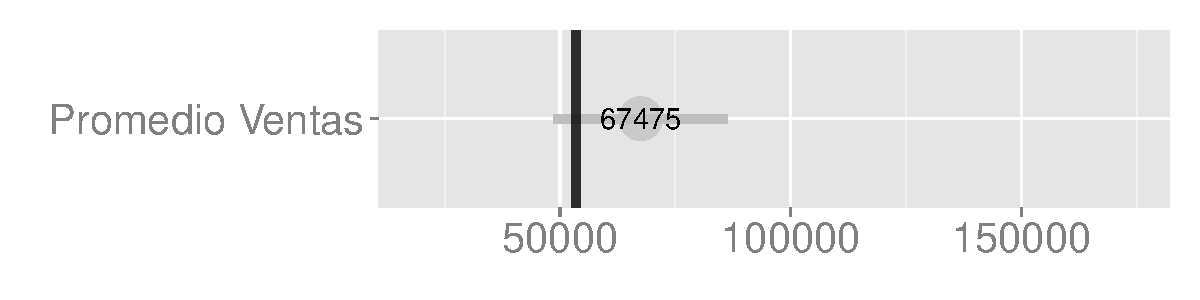
\includegraphics[width=10cm]{figure/unnamed-chunk-2} 

\end{knitrout}


\subsection*{Variables de entrada}

\begin{minipage}[b]{0.5\linewidth}
\begin{tabular}{r|r}
  \hline
 & x \\ 
  \hline
vehicular.s2.num & 300 \\ 
  generadores.totales & 60 \\ 
  poblacion & 20000 \\ 
  VIV28\_R & 80 \\ 
  VIV33\_R & 80 \\ 
  peatonal.s1.num & 300 \\ 
  VIV27\_R & 80 \\ 
  X24hrs & si \\ 
  SALUD1\_R & 80 \\ 
  vehicular.s1.num & 1000 \\ 
  VIV2\_R & 80 \\ 
  ubicacion & Esquina \\ 
  peatonal.s2.num & 120 \\ 
  VIV36\_R & 80 \\ 
  competencia.directa.total & 15 \\ 
  metros2 & 150 \\ 
  pdm.media.anual & 15 \\ 
  tipo.de.calle & Vehicular \\ 
  VIV35\_R & 80 \\ 
  corte & 53400 \\ 
  cajas & 3 o mas  \\ 
   \hline
\end{tabular}


\end{minipage}
\begin{minipage}[b]{0.3\linewidth}
\begin{knitrout}
\definecolor{shadecolor}{rgb}{0.969, 0.969, 0.969}\color{fgcolor}
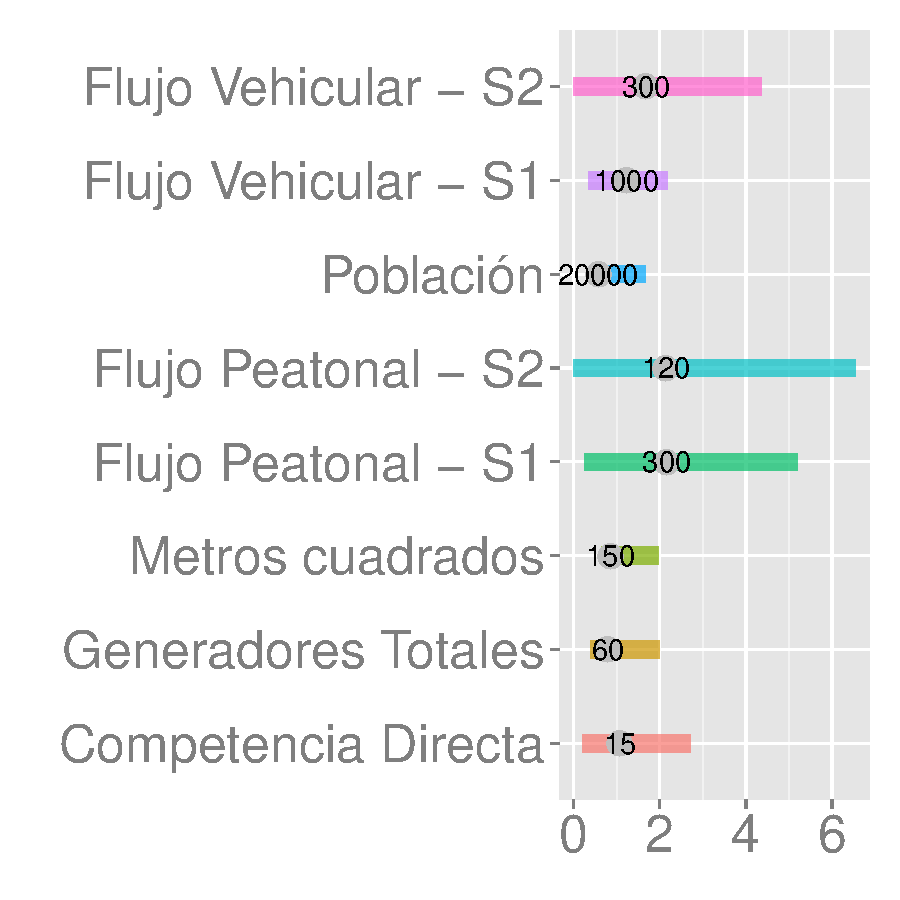
\includegraphics[width=6cm]{figure/unnamed-chunk-3} 

\end{knitrout}

\end{minipage}
\end{document}


